\documentclass[12pt]{article}

% import packages
\usepackage[utf8]{inputenc}
\usepackage{float}
\usepackage{subfloat}
\usepackage{subfig}
\usepackage{amsmath}
\usepackage[toc,page]{appendix}
\usepackage{caption}
\usepackage{graphicx}
\usepackage{hyperref}
\usepackage[left=1in,top=0.75in,right=1in,bottom=0.75in]{geometry}

\graphicspath{ {./images} }
% hyperref setup
\hypersetup{
	colorlinks=true,
	linkcolor=blue,
	filecolor=blue,      
	urlcolor=blue,
	citecolor=blue,
	pdftitle={Elastic beams lab report},
	pdfpagemode=FullScreen,
}
% titlepage	
\title{\textbf{Elastic beams lab report}}
\author{Callum Stephenson, css47}
\date{22nd February 2022}

\begin{document}
    \begin{titlepage}
        \maketitle
        \thispagestyle{empty}
        \vspace{13cm}
        \textbf{Department of Engineering, University of Cambridge}
    \end{titlepage}
    \newpage
    \section{Summary}
        Within this report, a beam is loaded by a point-load of 50N in order to understand the effects of bending on the curvature of a simply supported beam. The beam is kept within its elastic region
        so no plastic deformation occurs.
        The curvature values were gathered using a digital curvature gauge, which was calibrated on a larger wheel of known diameter. There was a "sanity check" measurement of the midpoint's vertical displacement
        also taken to compare against numerically integrated values. The results showed that the gathered data was consistent with theory, 
        and that the curvature linearly decreases from the centre until the supports, then beyond the supports there is no curvature as there is no capacity to carry moment. 

    \section{Introduction}
        The aim of this report is to investigate the nature of beams bending under a point load within the elastic region. These deflections are so 
        small that it is necessary to set up equipment to measure them precisely. 
        A device will be used to measure the local curvature of the beam rather than placing multiple displacement gauges along the length. \\ \\
        The way in which curvative is investigated is using a simply supported aluminium beam loaded in the midpoint. 
    \section{Laboratory setup}
        \subsection{Apparatus}
            Within this section, the equipment used within the laboratory will be listed with reasoning why it was chosen and a short summary of its functionality. \\
            The beam itself was an aluminium beam with notches every 5 centimetres, with notch 1 and 11 to be placed on a roller and pin joint respectively. This were to be
            placed into a loading frame. \\
            A curvature gauge was used in order to measure the local curvature at each of the 14 points in the beam. The curvature gauge was datumed on a known flat beam
            in order to remove zero error from the experiment. They were already previously calibrated on a large wheel of known curvature close to where they are stored.\\
            In order to measure the central displacement another separate displacement gauge was also required. There was no need to zero this as the measurement
            was simply a difference rather than an absolute with refenced to zero. \\
            A load stalk and 5 kilogram masses were required in order to achieve the desired load on the midpoint of the beam.
        \subsection{Testing methodology}
            Prior to adding any load to the setup, the initial curvature must be measured. The empty load stalk was added and the digital curvature gauge was 
            placed at each of the 14 points along the beam and a measurement was taken and recorded into a table. \\ After recording the pre-load curvature, 5 kilogram masses
            were added to the load stalk. The curvature was once again recorded at each of the 14 measurement points along the beam. Finally, once the midpoint displacement
            was measured with the load added using the displacement gauge, then the setup was unloaded and a second reading was taken. The difference between these
            two measurements was recorded - this is mainly to have a comparison for the calculation later.
    \section{Results, observation and calculations}
        The results were collated into a spreadsheet and python to graph the different quantities associated with the experiment. The calibration factor of the curvature found
        by comparing the measured to known curvature on a reference wheel. The gauge measured 0.01685 cm$^{-1}$ and the actual is 0.01666 cm$^{-1}$. This means that the
        gauge is off by a factor of 1.1\%, which is relatively accurate for what is required to be measured. The measured curvature against station number is shown below in 
        figure \ref{kappa_measured_station}.  The curvature is a linear increase until the maximum at the point where the load is applied, and rising back up to zero by time it the gauge is over
        the second support. There is no curvature past the support which is as expected as there is no continued bending moment.
        \begin{figure}[H]
            \centering
            \captionsetup{labelfont=bf}
            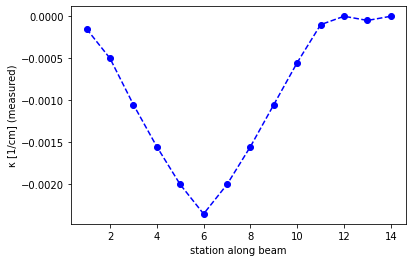
\includegraphics[width=20pc]{kappa_measured_station.png}
            \caption{Graph to show measured curvature values against station number}\label{kappa_measured_station}
        \end{figure}
        In order to calculate the moment in the beam it is possible to use a simple free body diagram as shown below.
        \begin{figure}[H]
            \centering
            \captionsetup{labelfont=bf}
            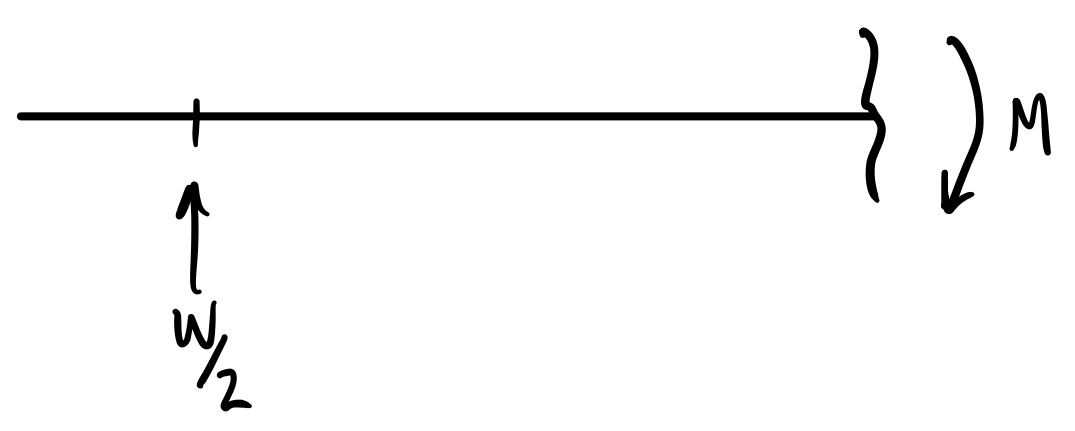
\includegraphics[width=15pc]{momentFBD.png}
            \caption{Moment FBD}\label{momentFBD}
        \end{figure}
        \begin{equation}
            M = \frac{W}{2}.x
        \end{equation}
        Where actual horizontal distance across the beam is approximated to just x ($S \approx X$). From this, it is possible to calculate M/B where B is obtained from the gradient
        of the experimental data shown in the figure below \ref{moment_kappa}. B was calculated to $\approx 2.4$x$10^{5}$ Nm$^{-2}$.
        \begin{figure}[H]
            \centering
            \captionsetup{labelfont=bf}
            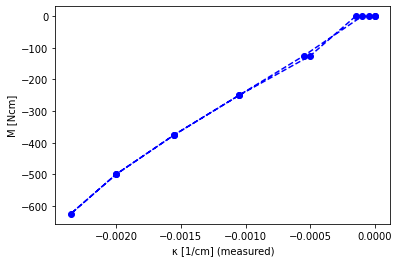
\includegraphics[width=20pc]{moment_kappa.png}
            \caption{Graph to show measured curvature values against calculated moment}\label{moment_kappa}
        \end{figure}
        The graphs of M and $\kappa$ are both linearly increasing until station 11, so it is expected that the graph of one against the other would form another linear
        graph. Using this calculated value of B, it is possible to use numerical integration in order to calculate the midpoint displacement. The value of B is relatively 
        close to reality as the graph of measured and simplfied kappa are close.
        \begin{figure}[H]
            \centering
            \captionsetup{labelfont=bf}
            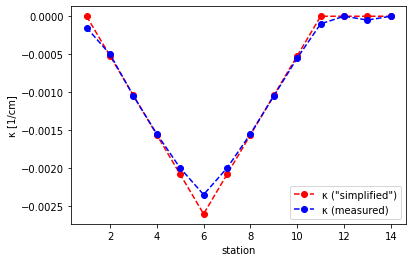
\includegraphics[width=20pc]{kappa_station_simplified.png}
            \caption{Graph to show measured curvature values against simplfied moment}\label{kappa_station_simplified}
        \end{figure}
        Integrating up twice and accounting for boundary conditions ($+c$ in integration) allows for a graph of y(vertical displacement) against stations to be formed. This can be
        compared to the measured value of midpoint displacement as during the laboratory session a midpoint measurement was gathered using the displacement gauge. The plot in 
        figure \ref{y_station_final} has the measured point plotted along with the calculated displacement.
        \begin{figure}[H]
            \centering
            \captionsetup{labelfont=bf}
            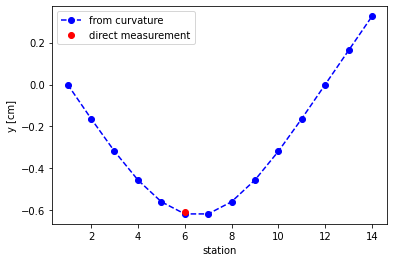
\includegraphics[width=20pc]{y_station_final.png}
            \caption{Graph to show displacement values(y), with a measured reference at station 6}\label{y_station_final}
        \end{figure}
        The curvature due to bending moment between stations 1-10 is as expected, and the linear region after 11 is expected as displacement = $R.\theta$ where theta is the angle
        at the support. The gradient of the displacement is 0 at the midpoint, which is expected as this is where the load was applied. It would still be possible to integrate
        given one of these boundary conditions was not available, such as under an asymmetrical deflections. 
    \section{Conclusion}
        The calculations of deflection using flexural stiffness yield comparable results to those found in the experiment within this report. The curvature also matches theory
        as it increases linearly until a maximum, then decreases steadily to zero from the support and beyond. This supports the original hypothesis that a point load produces
        curvature between two simply supported points, but as there is nothing to counteract moments beyond the support - this region will only have linear deflection and no
        curvature.
    \section{Discussion}
        The measured deflection is close to the calculated deflection (around 3\% error), so the calculations are relatively accurate for this one point. 
        Measuring just one point is not enough to justify saying that the deflection is valid throughout the whole beam, as there may be greater error within
        the other points along the beam. If the experiment were to be repeated, a minimum of 4 points of recorded displacement (excluding supports) would help to
        understand if the calculations made are valid for multiple sections of the beam. The calibration factor on the curvature gauge would have little effect 
        on the outcome of this experiment as the error was small. \\ \\
        One source of error within the experiment could be the assumption of g = 10 ms$^{-2}$ rather than the actual numerical value which could slightly chance the moments
        calculated, this in turn would chance the calculated value of flexural stiffness.
\end{document}